%%%%%%%%%%%%%%%%%%%%%%%%%%%%%%%%%%%%%%%%%%%%%%%%%%%%%%%%%%%%%%%%%%%%
\section{Organization and Management}
\label{sec:fdsp-slow-cryo-org}
% sowjanya

\fixme{structure under here is recommended}

%%%%%%%%%%%%%%%%%%%%%%%%%%%%%%%%%%%
\subsection{Slow Controls and Cryogenics Instrumentation Consortium Organization}
\label{sec:fdsp-slow-cryo-org-consortium}

% same in sp and dp

The organization of the CISC consortium is shown in
Fig.\ \ref{fig:sp-slow-cryo-org}. The CISC consortium board is
currently formed from institutional representatives from 16 institutes
as shown in Table \ref{tab:sp-slow-cryo-org}. The consortium leader
acts as the spokesperson for the consortium and is responsible for the
overall scientific program and management of the group. The technical
leader of the consortium is responsible for the project management for
the group.  Currently four working groups are envisioned in the
consortium (leaders to be appointed):

\begin{description}
 \item[Cryogenics Systems] gas analyzers, liquid level
  monitors and cryogenic internal piping
 \item[Liquid Argon Instrumentation] purity monitors, thermometers,
  cameras and light emitting system, and instrumentation test facility
 \item[Slow Controls Interfaces] signal processing software and
  hardware interfaces
 \item[Slow Controls Databases] alarms, archiving and monitoring GUIs
\end{description}

\begin{dunefigure}[CISC consortium organization]{fig:sp-slow-cryo-org}
{CISC Consortium organizational chart}
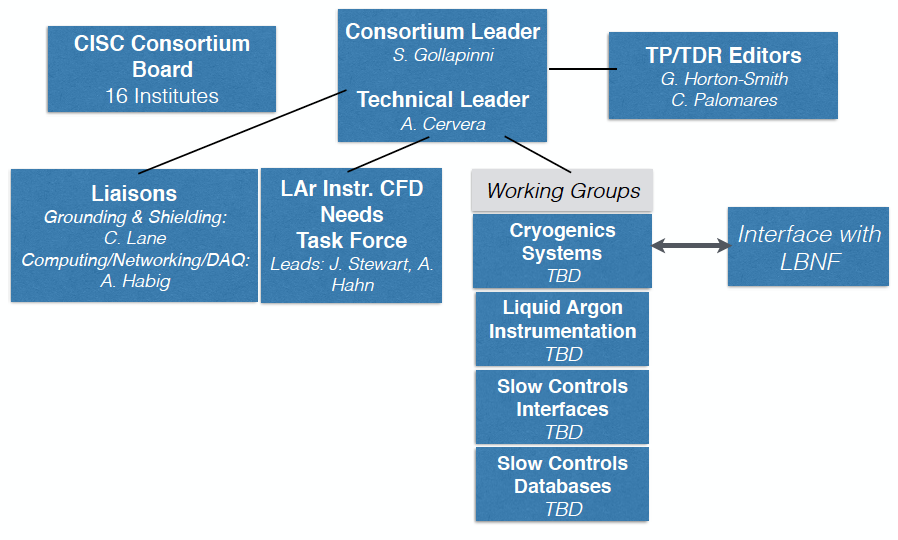
\includegraphics[width=0.7\textwidth]{fd-slow-cryo-org}
\end{dunefigure}

Additionally, since the CISC consortium broadly interfaces with other
groups, liaisons have been identified for various roles as listed in
Fig.\ \ref{fig:sp-slow-cryo-org}. A short-term focus group was
recently formed to understand the needs for cryogenic modeling for the
consortium. The Technical Proposal (TP) and Technical Design Report
(TDR) editors are responsible for the overall editing and delivery of
the TP/TDR documents to the collaboration. Currently members from new
institutes are added to the consortium based on consensus from the
consortium board members.

\begin{dunetable}
[CISC Consortium Institutions]
{p{0.3\textwidth}p{0.2\textwidth}p{0.3\textwidth}}
{tab:sp-slow-cryo-org}
{Current CISC Consortium Board Members and their institutional affiliations}
Member Institute  &  Country  &  Consortium Board Representative \\ \toprowrule
CIEMAT  &  Spain  &  Ines Gil Botella \\ \colhline
Instituto de Fisica Corpuscular  &  Spain  &  Anselmo Cervera \\ \colhline
University of Warwick  &  United Kingdom  &  Gary Barker \\ \colhline
University College London  &  United Kingdom  &  Mario Campanelli \\ \colhline
Argonne National Lab  &  USA  &  Jim Grudzinski  \\ \colhline
Brookhaven National Lab  &  USA  &  Jim Stewart \\ \colhline
University of California (Irvine)  &  USA  &  Jianming Bian \\ \colhline
Drexel University  &  USA  &  Charles Lane \\ \colhline
Fermi National Accelerator Lab  &  USA  &  Alan Hahn \\ \colhline
University of Hawaii  &  USA  &  Jelena Maricic \\ \colhline
University of Houston  &  USA  &  Andrew Renshaw \\ \colhline
Idaho State University  &  USA  &  Ed Tatar \\ \colhline
Kansas State University  &  USA  &  Glenn Horton-Smith \\ \colhline
University of Minnesota (Duluth)  &  USA  &  Alec Habig \\ \colhline
Notre Dame University  &  USA  &  John LoSecco \\ \colhline
University of Tennessee at Knoxville  &  USA  &  Sowjanya Gollapinni \\
\end{dunetable}


%%%%%%%%%%%%%%%%%%%%%%%%%%%%%%%%%%
\subsection{Planning Assumptions}
\label{sec:fdsp-slow-cryo-org-assmp}


%%%%%%%%%%%%%%%%%%%%%%%%%%%%%%%%%%%
\subsection{WBS and Responsibilities}
\label{sec:fdsp-slow-cryo-org-wbs}

%%%%%%%%%%%%%%%%%%%%%%%%%%%%%%%%%%
\subsection{High-level Cost and Schedule}
\label{sec:fdsp-slow-cryo-org-cs}
